\documentclass[11pt]{article}
\usepackage[ascii]{inputenc}
\usepackage{amsmath}
\usepackage{amssymb,amsfonts,textcomp}
\usepackage{bm}
\usepackage[T1]{fontenc}
\usepackage[english]{babel}
\usepackage{array}
\usepackage{supertabular}
\usepackage{hhline}
\usepackage{graphicx}
\usepackage{hyperref}
\usepackage{longtable}
\usepackage[table,xcdraw]{xcolor}
\usepackage{tabularx}
\usepackage{tabulary}
\usepackage{cite}

\usepackage{fancyhdr}
% For multi-line header, avoid sqquishing into main text
% https://tex.stackexchange.com/questions/162581/fancyhdr-adding-multiline-header-causes-footer-margin-to-be-inconsistent
\usepackage[
  headheight=38.82153pt, % height for the header block
]{geometry}

\usepackage{easyReview}
\usepackage{titlesec}  % for sub-sub-sub section

\newcommand{\adtversion}{0.1}
\newcommand{\adtversionname}{Version~\adtversion}
\newcommand{\adtreleaseshortname}{V\adtversion}
\newcommand{\adtdocumentid}{JPL D--108776}

\newcommand\signature[2]{ % name, title
\noindent\begin{minipage}{\textwidth}
    \noindent\vspace{0.5cm}\par
    \noindent\rule{\textwidth}{1pt}\par
    \noindent{#1}, {#2} \hfill Date\par
\end{minipage}}

% sub-sub-sub-sections
% https://tex.stackexchange.com/questions/60209/how-to-add-an-extra-level-of-sections-with-headings-below-subsubsection
\setcounter{secnumdepth}{4}
\titleformat{\paragraph}
{\normalfont\normalsize\bfseries}{\theparagraph}{1em}{}
\titlespacing*{\paragraph}
{0pt}{3.25ex plus 1ex minus .2ex}{1.5ex plus .2ex}


% header and footer

\pagestyle{fancy}
\fancyhf{}
\fancyhead[L]{\adtdocumentid \\ OPERA DIST-S1 ATBD}
\makeatletter
\fancyhead[R]{Initial Revision \\ \adtversionname\\
\@date}
\makeatother
\fancyfoot[C]{{\footnotesize
This document has been reviewed and determined not to contain export-controlled
data.\\
\hfil \normalsize{\thepage} \hfil
}}
%\fancyfoot[R]{\thepage}

\title{OPERA Algorithm Theoretical Basis Document for SAR Disturbance from RTC data}
% Observational Products for End-users from Remote sensing Analysis (OPERA) project
\author{Richard West, Charles Marshak, Talib Oliver Cabrera, Jungkyo Jung}
\def\today{\ifcase\month\or
  January\or February\or March\or April\or May\or June\or
  July\or August\or September\or October\or November\or December\fi
  \space\number\day, \number\year}
%\date{June 15, 2023 }
\date{\today}

\newcommand{\figtwosize}{2.5in}
\newcommand{\figonesize}{6.0in}
%\renewcommand{\headrulewidth}{0pt}
%\renewcommand{\footrulewidth}{0pt}
%\setlength\textheight{9.0in}
%\setlength\textwidth{6.0in}
%\setlength\oddsidemargin{0.1in}

\begin{document}

\makeatletter % get access to title, date, author macros
\begin{titlepage}
    \parindent0pt
    \vspace*{1cm}

    \includegraphics[width=3.5in]{fig/nasa-jpl-logo}

    \Huge
    \textbf{\@title}

    \vfill
    \Large

    \adtversionname

    \@date

    \vspace{0.5cm}

    \@author

    \vfill

    \footnotesize
    National Aeronautics and\\
    Space Administration

    Jet Propulsion Laboratory \\
    California Institute of Technology \\
    Pasadena, California

    \vfill
    {\footnotesize This document has been reviewed and determined not to contain export-controlled data. JPL/Caltech Proprietary Business Discreet. Caltech Record. Not for Public Distribution. Paper copies of this document may not be current and should not be relied on for official purposes. LRS number: LRR083444.}
    \thispagestyle{empty}

\end{titlepage}
\makeatother

%\maketitle
\thispagestyle{empty}
\newpage
\setcounter{page}{1}
\pagenumbering{roman}
\thispagestyle{fancy}

\thispagestyle{plain}

\noindent\Large\textbf{Signature Page}

\vspace{1cm}

\noindent\large\textbf{Prepared by:}
\normalsize

\signature{Richard West}{OPERA ADT/SAR-DIST-S1 Lead}
\signature{Charles Marshak}{OPERA ADT Engineer}
\signature{Talib Oliver Cabrera}{OPERA ADT Engineer}
\signature{Jungkyo Jung}{OPERA ADT/NISAR DSWx Lead}

\vfill

\noindent\large\textbf{Approved by:}
\normalsize

\signature{Steven Chan}{OPERA project scientist}
\signature{David Bekaert}{OPERA manager}

\vfill

% use header and footer on signature page
\thispagestyle{fancy}

\section*{Document Change Log}

% Please add the following required packages to your document preamble:
% \usepackage[table,xcdraw]{xcolor}


\begin{table}[!h]
\begin{tabular}
{
| p{0.15\linewidth} 
| p{0.12\linewidth}
| p{0.15\linewidth}
| p{0.1\linewidth}
| p{0.4\linewidth}
|
}
\hline
\rowcolor[HTML]{92A1CB} 
Revision & Cover Date  & Sections Changed & ECR \# & Reason, ECR Title, LRS \# \\ \hline
Initial & September 26, 2024 & All & N/A & New Document \\ \hline
%Preliminary & June 15, 2023 & All & N/A & New Document, LRR073167  \\ \hline
 &  &  &  &  \\ \hline
 &  &  &  &  \\ \hline
\end{tabular}
\end{table}

\section*{TBD/TBC Log}

% Please add the following required packages to your document preamble:
% \usepackage[table,xcdraw]{xcolor}


\begin{table}[!h]
\begin{tabular}
{
| p{0.15\linewidth} 
| p{0.5\linewidth}
| p{0.2\linewidth}
|
}
\hline
\rowcolor[HTML]{92A1CB} 
Section & Description & Due Date \\ \hline
 &  &   \\ \hline
 &  &   \\ \hline
 &  &   \\ \hline
\end{tabular}
\end{table}



\setcounter{tocdepth}{10}
\renewcommand\contentsname{}
\tableofcontents
\newpage

\setcounter{page}{1}
\pagenumbering{arabic}

\section{Introduction}

Within the OPERA disturbance product suite,
a radar-based surface disturbance product (DIST-S1)
is specified for release in early 2026.
Here, we develop the algorithm theoretical basis and describe this
new product to be derived from Sentinel-1A/C observations using
OPERA RTC products.

\section{DIST-S1 Algorithm Description}

The SAR disturbance algorithms considered here follow a signal based theme
as defined in the discussion of the optical disturbance algorithms
\cite{dist_hls_atbd}.
The primary inputs are the copolarized (VV) and cross-polarized (VH)
radar backscatter levels provided in the OPERA RTC products.
A disturbance is determined when the primary inputs are observed to change
by a signficant amount that lies outside of a measure of normal variation.
The determination of signficant change is applied at the 30 m posting
of the primary input RTC data.

The specific definition of significant change is considered in more
detail in the following subsection on Metric definitions.

\subsection{High Level Flow}

\begin{figure}[!t]
\centering
\includegraphics[width=\figonesize]{fig/high_level_flow.png}
\caption{High level flow of data when generating SAR Disturbance.}
\label{fig_high_level_flow}
\end{figure}

\subsection{Time Series Handling}

\subsection{RTC Loading and Preprocessing}

\subsection{Metric Definitions}

\subsubsection{LogRatio VH}
\subsubsection{Mahalonobis Distance 1D and 2D}
\subsubsection{LogRatio and Mahalonobis Distance}
\subsubsection{Transformer and Mahalonbis Distance}

\begin{figure}[!t]
\centering
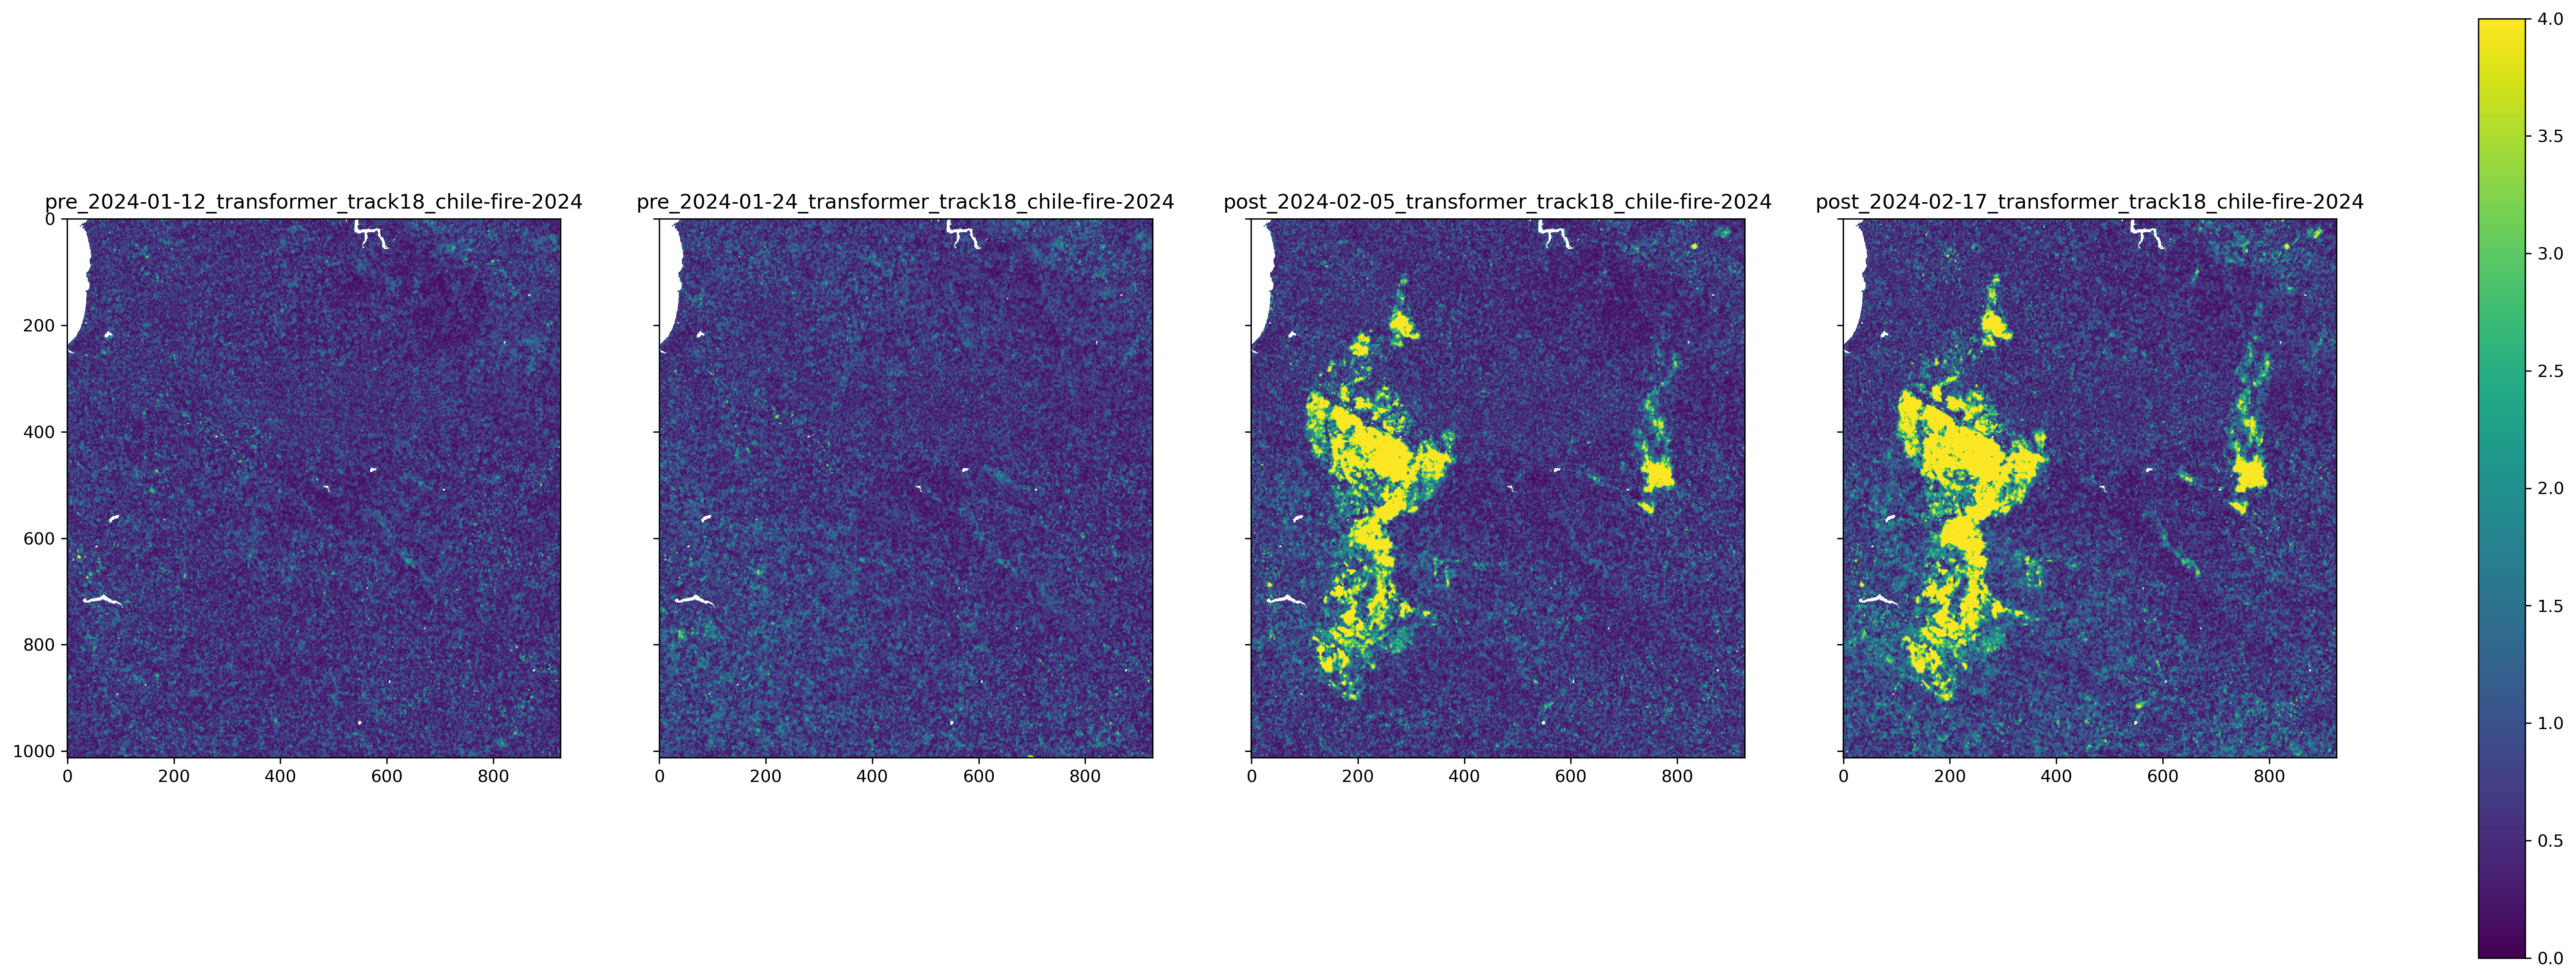
\includegraphics[width=\figonesize]{fig/transformer_metric_pre_post.png}
\caption{Comparison of Transformer Mahalonbis metric outputs for two
pre-event and two post-event scenes.}
\label{fig_transformer_metric_pre_post}
\end{figure}

\subsubsection{CuSum VH}
\subsubsection{CuSum Probability Max}

\subsection{Algorithm Inputs}

The main inputs to the algorithm are the latest RTC data take
along with prior RTC data takes that fall within a specified
prior time window.
The RTC data supply an orbit track of radar copolarized (VV)
and cross-polarized (VH) backscatter levels at 30 m posting.
These data come in burst order with overlap between bursts.
These radar backscatter levels are normalized to normal incidence
and ususally denoted $\gamma_0$.

In addition,
the algorithm uses two auxiliary products at different stages of
the processing flow.
A GLAD landcover classification mask is used to identify land areas,
and may be used to apply different threshold levels based on the landcover
classification.
An annual summary product serves as both input and output.
It is read to provide prior results from
this SAR Disturbance algorithm for the specific land area being processed.
These prior results are needed to determine confirmed disturbances.

\subsection{Algorithm Outputs}

The SAR Disturbance algorithm will output two types of products.
First, an ALERT product is generated corresponding to each new RTC track
of input data.
Second,
an annual summary product is updated based on the newly generated
ALERT product.
The ALERT product is a set of geotiff files,
each containing one layer of data as specified in table
\ref{table_output_layers}.
Each geotiff file contains one MGRS tile with 30 m posting,
following the same approach as the optical disturbance product
\cite{dist_hls_atbd}

\begin{table}[h]
\begin{center}
%\input table_output_layers.tex
\end{center}
\caption{Product Raster Layers for SAR-DIST-ALERT}
\label{table_output_layers}
\end{table}

\section{Algorithm Assumptions}

\section{Algorithm Implementation}

The OPERA DIST-S1 product workflow is developed by the OPERA
Algorithm Development Team (ADT).
It is implemented in Python and it is open-source accessed through the
following GitHub repository:
\noindent
https://github.com/opera-adt/DIST-S1

\section{Algorithm Usage Constraints}

\section{Performance Assessment}

\subsection{Validation Methods}

\subsubsection{DIST-HLS Test Sites}
\subsubsection{Ad-Hoc Test Scenes}

\subsection{Metric Performance and Downselection}

\subsubsection{LogRatio VH}
\subsubsection{Mahalonobis Distance 1D and 2D}
\subsubsection{LogRatio and Mahalonobis Distance}
\subsubsection{Transformer and Mahalonbis Distance}
\subsubsection{CuSum VH}
\subsubsection{CuSum Probability Max}

%\begin{figure}[!t]
%\centering
%\hbox{
%  \includegraphics[width=\figtwosize]{SEDel/bfpq_sim_raw_powers_hf.jpg}
%  \includegraphics[width=\figtwosize]{SEDel/bfpq_sim_raw_powers_vhf.jpg}
%  }
%\caption{Power levels during a 25 km Europa flyby.
%Left panel shows HF powers, right panel shows VHF powers which are a little
%lower than HF.}
%\label{fig_powers}
%\end{figure}

%\begin{figure}[!t]
%\centering
%\includegraphics[width=\figonesize]{SEDel/bfpq_sim_atten.jpg}
%\caption{Attenuator settings during a 25 km Europa flyby.}
%\label{fig_atten}
%\end{figure}

%\clearpage

\section{Data Access}
Data Access Input Data
\begin{itemize}
\item The primary input data to generate the DIST-S1 products,
are the RTC products which are available through the National
Aeronautics and Space Administration (NASA)
Alaska Satellite Facility (ASF)-Distributed Active Archive Center (DAAC).
\end{itemize}

Data Access Output Data:

\begin{itemize}
\item DIST-S1 products, will be made available through the National
Aeronautics and Space Administration (NASA)
Alaska Satellite Facility (ASF)-Distributed Active Archive Center (DAAC).
\end{itemize}
Data Access Related URLs

\section{Contacts}
% OPERA Algorithm Development Team

% \clearpage
% \section{Acronyms}
% \begin{longtable}{ll}
ADT & Algorithm Development Team \\
ASF & Alaska Satellite Facility \\
CSLC & Coregistered Single Look Complex \\
DAAC & Distributed Active Archive Center \\
DEM & Digital Elevation Model \\
ECEF & Earth-centered Earth-fixed \\
ECMWF & European Centre for Medium-Range Weather Forecasts \\
ERA5 & ECMWF Re-Analysis version 5 \\
ESA & European Space Agency \\
FM & Frequency Modulation \\
GIM & Global Ionospheric Maps \\
GNSS & Global Navigation Satellite System \\
GSLC & Geocoded Single-Look Complex \\
HDF5 & Hierarchical Data Format version 5 \\
IERS & International Earth Rotation and Reference System  \\
InSAR & Interferometric SAR \\
IPF & Instrument Processing Facility \\
IPP & Ionospheric Piercing Point \\
ISCE3 & InSAR Scientific Computing Environment version 3 \\
IW & Interferometric Wide (S1-A/B mode) \\
JPL & Jet Propulsion Laboratory \\
L1 & Level-1 product \\
L2 & Level-2 product \\
LOS & Line of Sight \\
LUT & Look-Up Table \\
MAGIC & Model-Adjusted Geometrical Image Coregistration \\
MAP & Maximum a Posteriori \\
NASA & National Aeronautics and Space Administration \\
NISAR & NASA-ISRO SAR \\
PRF & Pulse Repetition Frequency \\
PRI  & Pulse Repetition Interval \\
OPERA & Operational Product for End-users from Remote sensing Analysis \\
RFI & Radio Frequency Interference \\
RSF & Range Sampling Frequency \\
S1 & Sentinel-1 \\
S1-A/B & Sentinel-1 A/B \\
SAR & Synthetic Aperture Radar \\
ScanSAR & Scanning Synthetic Aperture Radar \\
SET & Solid Earth Tides \\
SLC & Single-Look Complex \\
SNAPHU & Statistical-cost Network-flow Algorithm for PHase Unwrapping \\
SNR & Signal-to-Noise ratio \\
TEC & Total Electron Content \\
TECU & TEC Unit \\
TOPS & Terrain Observation with Progressive Scan \\
VTEC & Vertical TEC \\
WGS84 & World Geodetic System 1984 \\
XML & eXtensible Markup Language \\
\end{longtable}
% \clearpage
\section{Acronyms}

\begin{longtable}{ll}
ADT & Algorithm Development Team \\
ASF & Alaska Satellite Facility \\
CSLC & Coregistered Single Look Complex \\
DAAC & Distributed Active Archive Center \\
DEM & Digital Elevation Model \\
ECEF & Earth-centered Earth-fixed \\
ECMWF & European Centre for Medium-Range Weather Forecasts \\
ERA5 & ECMWF Re-Analysis version 5 \\
ESA & European Space Agency \\
FM & Frequency Modulation \\
GIM & Global Ionospheric Maps \\
GNSS & Global Navigation Satellite System \\
GSLC & Geocoded Single-Look Complex \\
HDF5 & Hierarchical Data Format version 5 \\
IERS & International Earth Rotation and Reference System  \\
InSAR & Interferometric SAR \\
IPF & Instrument Processing Facility \\
IPP & Ionospheric Piercing Point \\
ISCE3 & InSAR Scientific Computing Environment version 3 \\
IW & Interferometric Wide (S1-A/B mode) \\
JPL & Jet Propulsion Laboratory \\
L1 & Level-1 product \\
L2 & Level-2 product \\
LOS & Line of Sight \\
LUT & Look-Up Table \\
MAGIC & Model-Adjusted Geometrical Image Coregistration \\
MAP & Maximum a Posteriori \\
NASA & National Aeronautics and Space Administration \\
NISAR & NASA-ISRO SAR \\
PRF & Pulse Repetition Frequency \\
PRI  & Pulse Repetition Interval \\
OPERA & Operational Product for End-users from Remote sensing Analysis \\
RFI & Radio Frequency Interference \\
RSF & Range Sampling Frequency \\
S1 & Sentinel-1 \\
S1-A/B & Sentinel-1 A/B \\
SAR & Synthetic Aperture Radar \\
ScanSAR & Scanning Synthetic Aperture Radar \\
SET & Solid Earth Tides \\
SLC & Single-Look Complex \\
SNAPHU & Statistical-cost Network-flow Algorithm for PHase Unwrapping \\
SNR & Signal-to-Noise ratio \\
TEC & Total Electron Content \\
TECU & TEC Unit \\
TOPS & Terrain Observation with Progressive Scan \\
VTEC & Vertical TEC \\
WGS84 & World Geodetic System 1984 \\
XML & eXtensible Markup Language \\
\end{longtable}

\section{Acknowledgements}
This research was conducted at the Jet Propulsion Laboratory,
California Institute of Technology, under contract with
the National Aeronautics and Space Administration.

The original Copernicus Sentinel data used for this paper have been provided by the European Space Agency.

\begin{thebibliography}{3}

\bibitem{dist_hls_atbd}
M. C. Hansen, A. Pickens, Z. Song,
\emph{OPERA DIST product},
https://lpdaac.usgs.gov/documents/1835/OPERA\_DIST\_ATBD\_\_V1.pdf
%\bibitem{scuccato2018}
%T. Scuccato,
%\emph{N-bit quantization and N-bit Block Floating Point Quantization analysis
%for radar sounder application},
%JPL Internal document, docushare collection 270622, June 2018.
\end{thebibliography}

\end{document}


